\section{ТЕОРЕТИЧЕСКИЕ ОСНОВЫ ТЕХНОЛОГИИ BLUETOOTH И ТРЕБОВАНИЯ К СТЕНДУ}

\subsection{История развития и архитектурные особенности Bluetooth (BR/EDR и BLE)}

Технология беспроводной передачи данных Bluetooth была представлена шведской компанией Ericsson в 1994 году как решение для замены кабельных соединений между мобильными телефонами и аксессуарами~\cite{bluetooth_history}. Название технологии происходит от прозвища датского короля Харальда I Синезубого (Harald Blåtand), который объединил разрозненные датские племена в единое королевство в X веке. Аналогично этому технология Bluetooth была призвана объединить различные коммуникационные протоколы и устройства в единую беспроводную экосистему.

В 1998 году ведущие технологические компании Ericsson, IBM, Intel, Nokia и Toshiba образовали консорциум Bluetooth Special Interest Group (Bluetooth SIG), который занимается развитием стандарта и сертификацией устройств. Первая спецификация Bluetooth 1.0 была опубликована в 1999 году, а первые коммерческие устройства появились на рынке в 2000 году.

\begin{figure}[H]
\centering
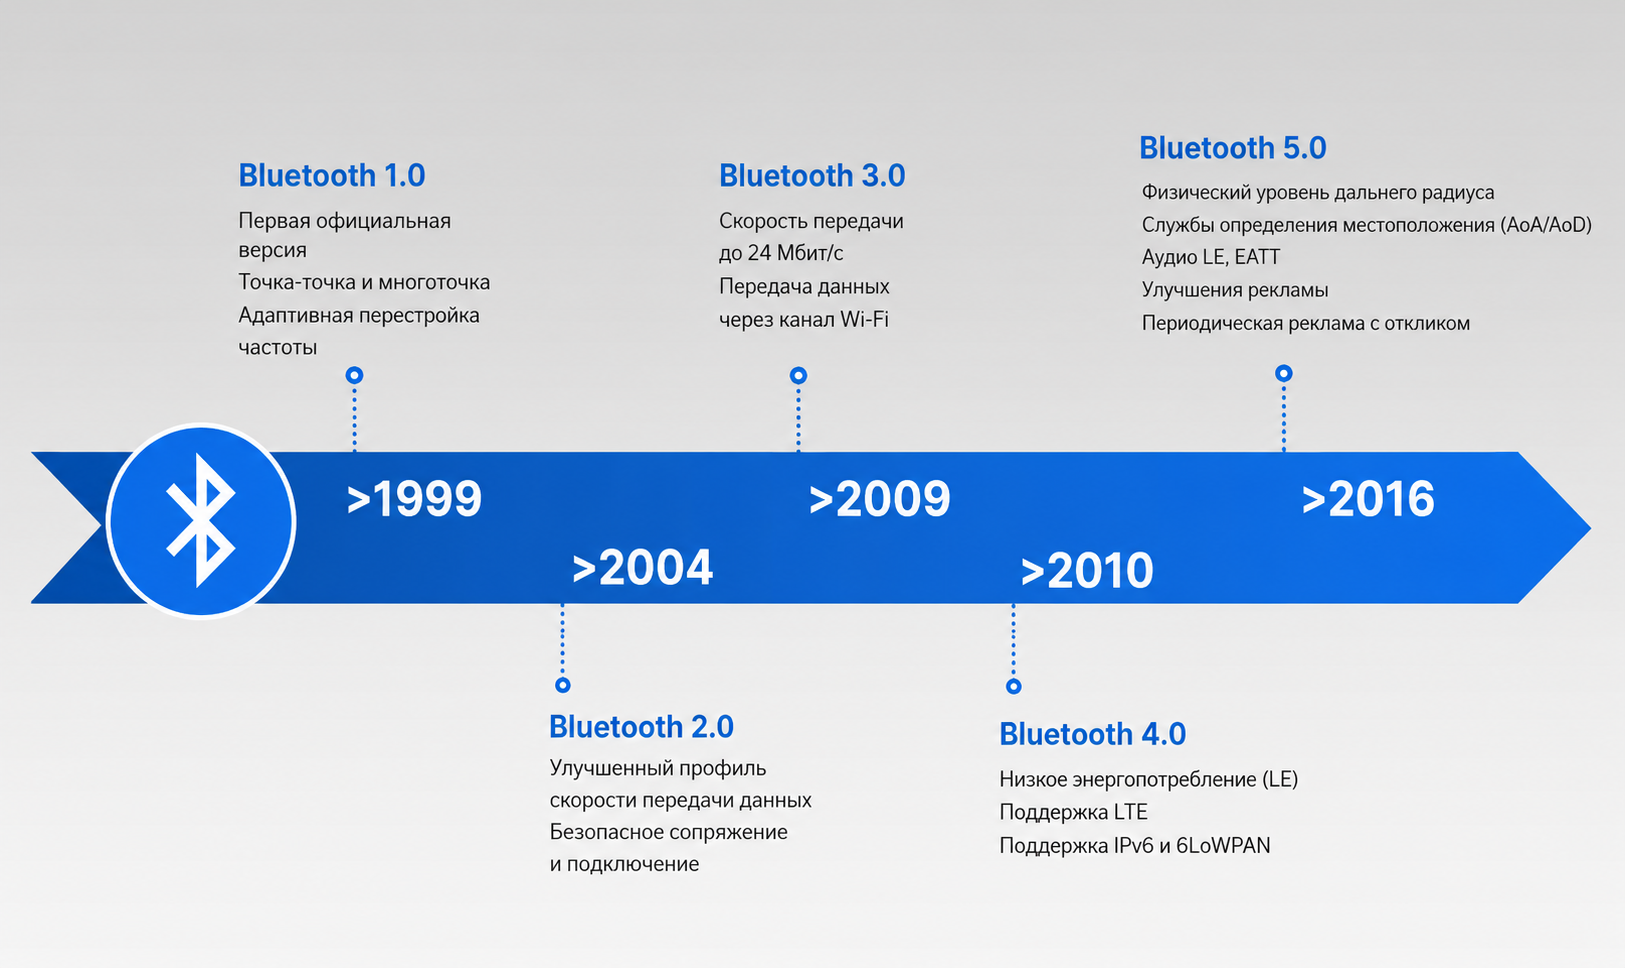
\includegraphics{figures/bluetooth_timeline.png}
\caption{Временная шкала развития версий Bluetooth}
\label{fig:bluetooth_timeline}
\end{figure}

За более чем три десятилетия развития технология Bluetooth претерпела значительные изменения. Были выпущены многочисленные версии спецификации, каждая из которых привносила улучшения в скорость передачи данных, дальность связи, энергоэффективность и функциональность. Ключевыми вехами стали:
\begin{itemize}[nosep]
    \item \textbf{Bluetooth 1.x (1999--2003)} --- первые версии с базовой скоростью передачи данных 1 Мбит/с;
    \item \textbf{Bluetooth 2.0 + EDR (2004)} --- введение режима Enhanced Data Rate (EDR) с увеличением скорости до 3 Мбит/с;
    \item \textbf{Bluetooth 3.0 + HS (2009)} --- поддержка High Speed через альтернативный MAC/PHY (обычно Wi-Fi);
    \item \textbf{Bluetooth 4.0 (2010)} --- революционное обновление с введением Bluetooth Low Energy (BLE) как отдельного протокола;
    \item \textbf{Bluetooth 5.0 (2016)} --- увеличение дальности связи в 4 раза и скорости в 2 раза по сравнению с Bluetooth 4.x;
    \item \textbf{Bluetooth 5.3 (2021)} --- версия с улучшениями в области безопасности, стабильности соединения и эффективности использования спектра~\cite{bluetooth_core53}.
\end{itemize}

Современная спецификация Bluetooth Core Specification 5.3 определяет два основных типа радиотехнологий, которые хотя и используют один и тот же диапазон частот, имеют существенные архитектурные различия.

\subsubsection{Классический Bluetooth (BR/EDR)}

\textbf{BR/EDR (Basic Rate / Enhanced Data Rate)} --- это оригинальная технология Bluetooth, также называемая классическим Bluetooth. Она оптимизирована для приложений, требующих непрерывной передачи данных с относительно высокой скоростью, таких как потоковая передача аудио, передача файлов или эмуляция последовательных портов.

\begin{figure}[H]
\centering
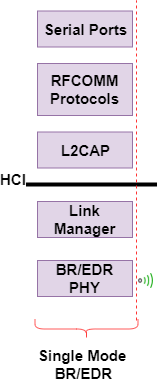
\includegraphics{figures/bredr_stack.png}
\caption{Стек протоколов классического Bluetooth BR/EDR}
\label{fig:bredr_stack}
\end{figure}

Архитектура BR/EDR включает следующие ключевые компоненты:
\begin{enumerate}[nosep]
    \item \textbf{Радиоуровень (Radio)} --- работает в нелицензируемом ISM-диапазоне 2{,}4--2{,}4835 ГГц, используя схему модуляции Gaussian Frequency Shift Keying (GFSK) для базовой скорости и $\pi/4$-DQPSK, 8DPSK для режима EDR. Спектр разделён на 79 каналов с шагом 1 МГц.

    \item \textbf{Уровень Baseband} --- отвечает за формирование пакетов, управление доступом к среде, синхронизацию и установление соединений. Использует технику скачкообразной перестройки рабочей частоты Frequency Hopping Spread Spectrum (FHSS) со скоростью 1600 хоппингов в секунду для повышения помехоустойчивости.

    \item \textbf{Протокол LMP (Link Manager Protocol)} --- управляет установлением соединения, аутентификацией, шифрованием, согласованием параметров канала и управлением энергосбережением между устройствами Bluetooth.

    \item \textbf{Интерфейс HCI (Host Controller Interface)} --- стандартизированный программно-аппаратный интерфейс между хостом (операционная система, драйвер или стек Bluetooth) и Bluetooth-контроллером. HCI определяет формат команд, событий и пакетов данных, обеспечивая независимость программной части от конкретной аппаратной реализации адаптера. Через HCI выполняются операции поиска устройств, установления соединений, управления шифрованием и передачи ACL/SCO-пакетов.

    \item \textbf{Протокол L2CAP (Logical Link Control and Adaptation Protocol)} --- обеспечивает мультиплексирование нескольких логических соединений поверх одного физического канала, сегментацию и реассемблирование пакетов, а также управление качеством обслуживания (QoS).

    \item \textbf{Профили и протоколы верхнего уровня} --- включают RFCOMM (эмуляция последовательного порта), SDP (Service Discovery Protocol), A2DP (Advanced Audio Distribution Profile), HFP (Hands-Free Profile) и другие профили, определяющие конкретные сценарии использования Bluetooth.
\end{enumerate}

Классический Bluetooth обеспечивает скорость передачи данных до 3 Мбит/с (EDR) и поддерживает два типа соединений:
\begin{itemize}[nosep]
    \item \textbf{SCO (Synchronous Connection-Oriented)} --- симметричное соединение с фиксированной полосой пропускания для передачи голосового трафика;
    
    \item \textbf{ACL (Asynchronous Connection-Link)} --- асимметричное пакетное соединение для передачи пользовательских данных.
\end{itemize}

\subsubsection{Профили классического Bluetooth (BR/EDR)}

Профили Bluetooth представляют собой стандартизированные наборы протоколов и правил взаимодействия, определяющие конкретные сценарии использования технологии. Для классического Bluetooth (BR/EDR) разработан широкий набор профилей, обеспечивающих совместимость устройств различных производителей.

Основные профили BR/EDR включают:
\begin{itemize}[nosep]
    \item \textbf{SPP (Serial Port Profile)} --- эмуляция последовательного интерфейса RS-232, широко используется для передачи данных между устройствами;
    
    \item \textbf{HID (Human Interface Device)} --- поддержка устройств ввода, таких как клавиатуры, мыши и игровые контроллеры;
    
    \item \textbf{A2DP (Advanced Audio Distribution Profile)} --- передача стереофонического аудиопотока на беспроводные наушники и акустические системы;
    
    \item \textbf{AVRCP (Audio/Video Remote Control Profile)} --- управление воспроизведением мультимедиа (громкость, переключение треков);
    
    \item \textbf{HFP (Hands-Free Profile)} --- организация голосовой связи в автомобильных системах и гарнитурах;
    
    \item \textbf{OPP (Object Push Profile)} --- передача файлов между устройствами;
    
    \item \textbf{FTP (File Transfer Profile)} --- доступ к файловой системе удалённого устройства.
\end{itemize}

Использование профилей позволяет абстрагироваться от низкоуровневых особенностей протоколов и обеспечивает интероперабельность устройств в различных прикладных сценариях.

\subsubsection{Bluetooth Low Energy (BLE)}

\textbf{Bluetooth Low Energy (BLE)}, также известный как Bluetooth Smart, был представлен в спецификации Bluetooth 4.0 в 2010 году как технология, оптимизированная для приложений с низким энергопотреблением и эпизодической передачей небольших объёмов данных~\cite{ble_intro}. BLE не является просто энергосберегающей версией классического Bluetooth --- это принципиально иная технология с упрощённой архитектурой, разработанная с нуля.

\begin{figure}[H]
\centering
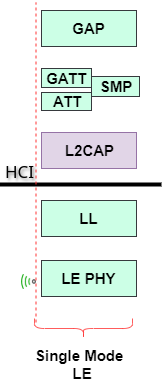
\includegraphics{figures/ble_stack.png}
\caption{Стек протоколов Bluetooth Low Energy}
\label{fig:ble_stack}
\end{figure}

Архитектурные особенности BLE включают:
\begin{enumerate}[nosep]
    \item \textbf{Упрощённый радиоуровень} --- использует 40 каналов с шагом 2 МГц, из которых 3 канала зарезервированы для advertising и установления соединения, а 37 используются для передачи данных. Модуляция GFSK с индексом 0{,}5 обеспечивает скорость передачи 1 Мбит/с.

    \item \textbf{Протокол Link Layer} --- реализует пять состояний устройства: Standby, Advertising, Scanning, Initiating и Connected. Это позволяет устройствам большую часть времени находиться в спящем режиме.

    \item \textbf{Протокол ATT (Attribute Protocol)} --- определяет клиент-серверную модель взаимодействия, где данные представляются в виде атрибутов, организованных в службы.

    \item \textbf{Протокол GATT (Generic Attribute Profile)} --- надстройка над ATT, определяющая процедуры обнаружения служб, чтения и записи характеристик, а также механизм уведомлений и индикаций.

    \item \textbf{Протокол GAP (Generic Access Profile)} --- управляет процедурами обнаружения устройств, установления соединения и безопасности.

    \item \textbf{SM (Security Manager)} --- обеспечивает генерацию и обмен ключами шифрования, аутентификацию устройств.
\end{enumerate}

\subsubsection{Профили и службы Bluetooth Low Energy (BLE)}

В Bluetooth Low Energy концепция профилей реализована через модель служб и характеристик, основанную на протоколе GATT. В отличие от классического Bluetooth, BLE использует более лёгковесную и гибкую архитектуру, ориентированную на передачу небольших объёмов данных.

Профили BLE определяются как наборы служб (services), каждая из которых содержит характеристики (characteristics), представляющие данные и методы взаимодействия с ними.

К основным стандартным службам BLE относятся:
\begin{itemize}[nosep]
    \item \textbf{Generic Access (GAP)} --- определяет параметры обнаружения устройств, установления соединения и роли (central/peripheral);
    
    \item \textbf{Generic Attribute (GATT)} --- обеспечивает структуру обмена данными между клиентом и сервером;
    
    \item \textbf{Device Information Service} --- предоставляет информацию об устройстве (производитель, версия, идентификаторы);
    
    \item \textbf{Battery Service} --- передача информации об уровне заряда батареи;
    
    \item \textbf{Heart Rate Service} --- используется в медицинских и спортивных устройствах для передачи данных о частоте сердечных сокращений;
    
    \item \textbf{Environmental Sensing Service} --- применяется для передачи данных с датчиков окружающей среды (температура, влажность и др.).
\end{itemize}

Помимо стандартных профилей, BLE допускает создание пользовательских (custom) служб, что делает технологию особенно гибкой для применения в системах Интернета вещей.

Таким образом, BLE ориентирован на модель клиент--сервер с использованием атрибутов, в то время как классический Bluetooth использует более жёстко определённые профили взаимодействия.

\subsubsection{Сравнительный анализ BR/EDR и BLE}

Несмотря на использование общего диапазона частот и принадлежность к единому стандарту, BR/EDR и BLE имеют фундаментальные различия, представленные в таблице~\ref{tab:ble_bredr_compare}.

\begin{table}[H]
\centering
\caption{Сравнение характеристик Bluetooth LE (BLE) и Bluetooth BR/EDR}
\label{tab:ble_bredr_compare}
\renewcommand{\arraystretch}{1.3}

\begin{tabularx}{\textwidth}{|X|X|X|}
\hline
\textbf{Характеристика} & \textbf{Bluetooth LE (BLE)} & \textbf{Bluetooth BR/EDR} \\
\hline

Диапазон частот &
2{,}4 ГГц &
2{,}4 ГГц \\
\hline

Каналы &
40 каналов с шагом 2 МГц \newline
(3 advertising-канала / 37 каналов данных)$^{1}$ &
79 каналов с шагом 1 МГц \\
\hline

Использование каналов &
FHSS &
FHSS \\
\hline

Модуляция &
GFSK &
GFSK, $\frac{\pi}{4}$ DQPSK, 8DPSK \\
\hline

Максимальная скорость передачи &
2 Мбит/с &
3 Мбит/с \\
\hline

Максимальная мощность передачи &
100 мВт &
100 мВт \\
\hline

Энергопотребление &
$(0.01 \div 0.05)\cdot(1)^{2}$ &
$(1)^{2}$ \\
\hline

Топология сети &
Point-to-Point,$^{3}$ \newline
Broadcast, Mesh &
Point-to-Point,$^{3}$ \newline
Scatternet \\
\hline

Тип соединения &
Кратковременная пакетная передача данных &
Непрерывный поток данных \\
\hline

Типичная дальность &
30 м &
50 м \\
\hline

\end{tabularx}

\vspace{0.3cm}

\begin{flushleft}
\footnotesize
$^{1}$ Advertising-каналы: ch.~37 (2402 МГц), ch.~38 (2426 МГц), ch.~39 (2480 МГц). \\
$^{2}$ Значение (1) принято за опорное. \\
$^{3}$ Включая пикосеть (piconet).
\end{flushleft}

\end{table}

Современные устройства, такие как микроконтроллер ESP32, поддерживают одновременную работу обоих стеков (dual-mode), что позволяет гибко выбирать оптимальный протокол в зависимости от поставленной задачи~\cite{esp32_bt}.

\begin{figure}[H]
\centering
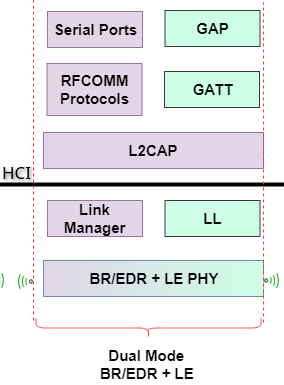
\includegraphics{figures/bredr_ble_stack.png}
\caption{Стек протоколов bluetooth dual-mode}
\label{fig:bredr_ble_stack}
\end{figure}

В рамках разрабатываемого лабораторного стенда это даёт возможность исследовать как классические сценарии использования Bluetooth, так и современные применения BLE в системах Интернета вещей.

Важно отметить, что начиная с Bluetooth 5.0 спецификация включает дополнительные режимы для BLE:
\begin{itemize}[nosep]
    \item \textbf{LE 2M PHY} --- удвоенная скорость передачи (2 Мбит/с);
    \item \textbf{LE Long Range} --- увеличенная дальность за счёт кодирования с коррекцией ошибок;
    \item \textbf{LE Advertising Extensions} --- расширенные возможности рекламы для поддержки mesh-сетей.
\end{itemize}

Эти улучшения делают BLE привлекательной технологией для широкого спектра приложений, включая системы позиционирования внутри помещений, носимую электронику и промышленные сети датчиков.

\subsection{Топологии Bluetooth-сетей: точка--точка, пикосеть, скаттернет}

Технология Bluetooth поддерживает несколько базовых топологий построения сетей, определяющих способы взаимодействия между устройствами и организацию обмена данными. Выбор конкретной топологии зависит от решаемых задач, количества устройств и требований к производительности сети. Спецификация Bluetooth определяет три основные топологии: соединение точка--точка (Point-to-Point), пикосеть (Piconet) и скаттернет (Scatternet).

\subsubsection{Соединение точка--точка}

Соединение точка--точка представляет собой простейшую форму организации связи в Bluetooth-сетях и предполагает непосредственное взаимодействие между двумя устройствами. В данной топологии одно устройство выступает в роли ведущего (master), а другое --- в роли ведомого (slave).

Характерные особенности топологии точка--точка:
\begin{enumerate}[nosep]
    \item \textbf{Прямая связь} --- устройства обмениваются данными непосредственно друг с другом без участия промежуточных узлов.

    \item \textbf{Выделенный канал} --- всё доступное время радиоэфира и полоса пропускания используются исключительно для связи между данной парой устройств, что обеспечивает максимальную производительность соединения.

    \item \textbf{Простота установления соединения} --- процедуры сопряжения и установления связи минимальны по сравнению с более сложными топологиями.

    \item \textbf{Гибкость ролей} --- устройства могут изменять роли master/slave в процессе работы, хотя в классическом Bluetooth роль ведущего обычно фиксируется при установлении соединения.
\end{enumerate}

Топология точка--точка используется в следующих сценариях:
\begin{itemize}[nosep]
    \item подключение беспроводной гарнитуры к мобильному телефону;
    \item передача файлов между двумя устройствами;
    \item подключение клавиатур и мышей к компьютеру;
    \item потоковая передача аудио.
\end{itemize}

\subsubsection{Пикосеть}

Пикосеть (Piconet) является основной формой организации Bluetooth-сетей. Она представляет собой сеть, состоящую из одного ведущего устройства и нескольких ведомых устройств, синхронизированных по общим часам и использующих единую последовательность скачкообразной перестройки частоты.

Основные характеристики пикосети:
\begin{enumerate}[nosep]
    \item \textbf{Количество устройств} --- пикосеть может включать одно ведущее устройство и до семи активных ведомых устройств одновременно. Дополнительно могут присутствовать припаркованные устройства (parked devices).

    \item \textbf{Роль ведущего устройства} --- ведущее устройство формирует сигналы синхронизации, определяет последовательность FHSS и управляет распределением временных слотов между ведомыми устройствами.

    \item \textbf{Роль ведомых устройств} --- ведомые устройства синхронизируются с ведущим по его часам и частотной последовательности. Каждому устройству назначается временный адрес AM\_ADDR длиной 3 бита.

    \item \textbf{Ограничение взаимодействия} --- обмен данными между двумя ведомыми устройствами напрямую невозможен; все данные передаются через master-устройство.
\end{enumerate}

Режимы работы ведомых устройств:
\begin{itemize}[nosep]
    \item \textbf{Active} --- устройство активно участвует в обмене данными;
    \item \textbf{Sniff} --- устройство периодически прослушивает эфир для экономии энергии;
    \item \textbf{Hold} --- временное прекращение передачи данных при сохранении синхронизации;
    \item \textbf{Park} --- устройство освобождает AM\_ADDR, оставаясь синхронизированным с пикосетью.
\end{itemize}

\subsubsection{Организация доступа к среде}

В технологии Bluetooth доступ к общей радиосреде в пикосети организуется на основе временного разделения каналов (TDMA) в сочетании со скачкообразной перестройкой частоты (FHSS). В соответствии с алгоритмом FHSS несущая частота изменяется до 1600 раз в секунду, а время передачи разбивается на интервалы (слоты) длительностью 625 мкс~\cite{bluetooth_core53}.

Каждый слот соответствует передаче данных на определённой частоте, причём последовательность смены частот является псевдослучайной и определяется параметрами ведущего устройства (его адресом и часами). Это позволяет нескольким пикосетям сосуществовать в одном диапазоне без существенных взаимных помех.

Обмен данными в пикосети осуществляется под управлением ведущего устройства, которое формирует сигналы синхронизации и управляет доступом к среде. Передача организована по принципу чередования слотов: ведущее устройство передаёт в одном слоте, а ведомое — в следующем. Ведомое устройство может начать передачу только после получения пакета от ведущего, адресованного именно ему.

Передача данных осуществляется пакетами, которые могут занимать один или несколько временных слотов. В случае завершения передачи до окончания слота происходит синхронная смена рабочей частоты.

Bluetooth поддерживает два типа логических соединений на уровне Baseband:
\begin{enumerate}[nosep]
    \item \textbf{SCO (Synchronous Connection-Oriented)} --- синхронные соединения с установлением связи, предназначенные для передачи изохронного трафика (например, аудио). Для таких соединений заранее резервируются временные слоты с фиксированной периодичностью. Передача осуществляется без повторов при ошибках, что обеспечивает постоянную задержку.

    \item \textbf{ACL (Asynchronous Connection-Less)} --- асинхронные пакетные соединения, реализующие обмен данными по схеме «ведущий--ведомые». Используются для передачи данных с возможностью адресации отдельных устройств или широковещательной передачи. В отличие от SCO, поддерживается повторная передача пакетов при обнаружении ошибок.
\end{enumerate}

\subsubsection{Скаттернет}

Скаттернет (Scatternet) представляет собой объединение нескольких пикосетей в единую сеть. Такая топология позволяет увеличить количество устройств и расширить покрытие сети.

\begin{figure}[H]
\centering
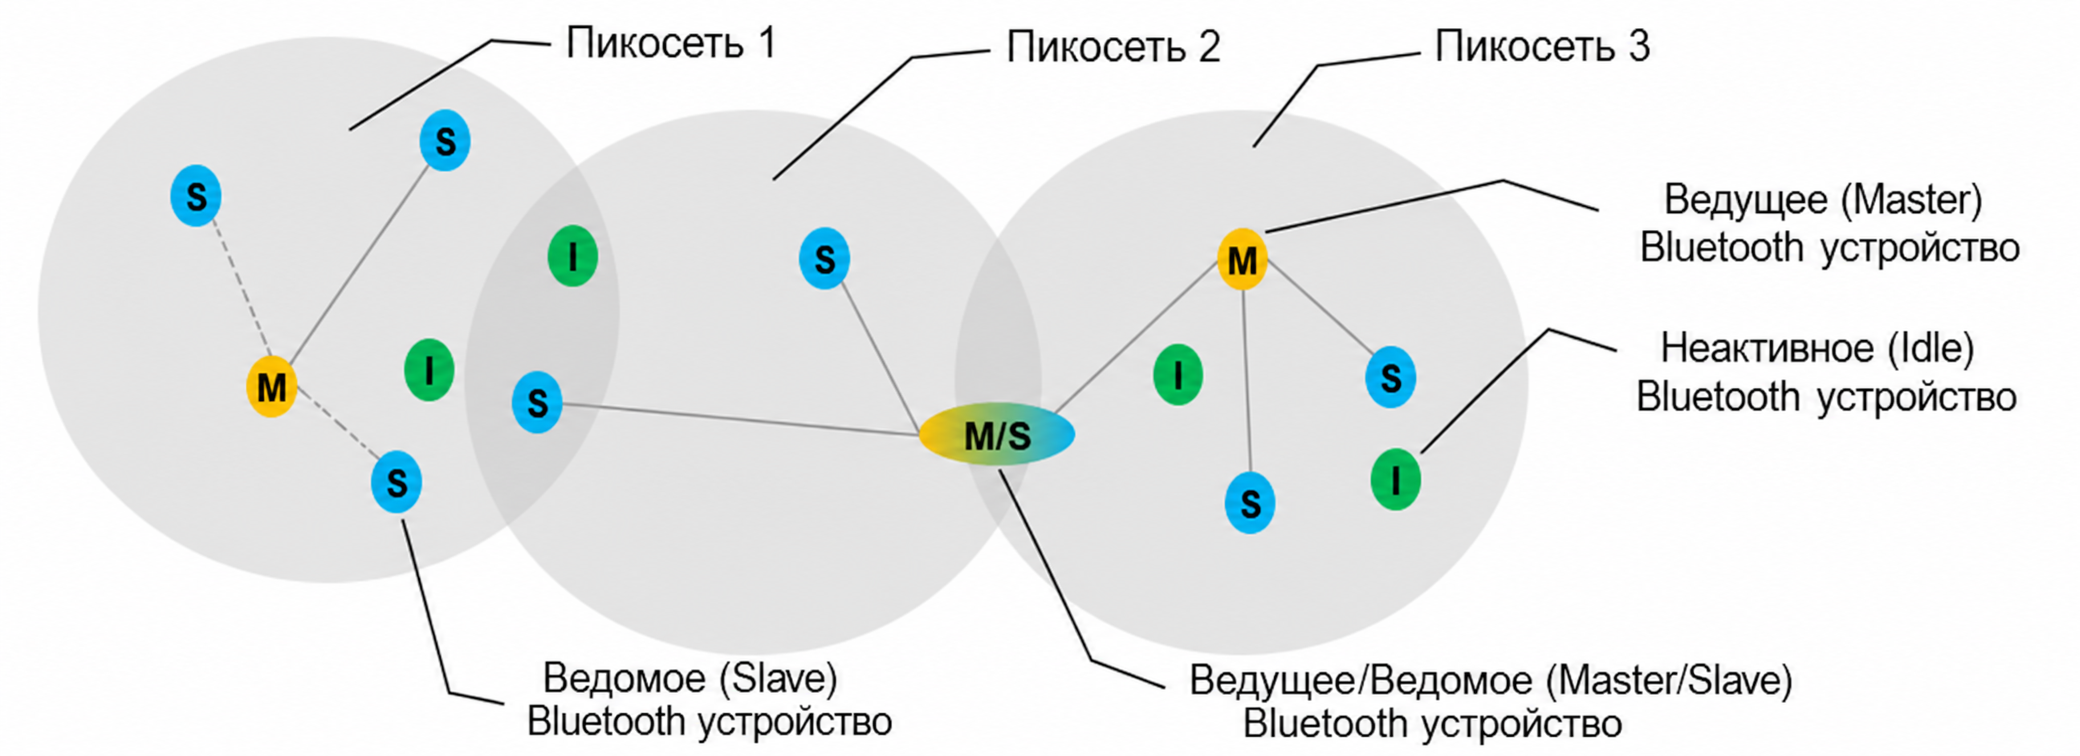
\includegraphics{figures/piconet_structure.png}
\caption{Структура скаттернета}
\label{fig:scatternet}
\end{figure}

Скаттернет формируется, когда одно или несколько устройств одновременно участвуют в нескольких пикосетях. Такие устройства называются PMP (Piconet Multiple Participation) или мостами (bridges).

Устройство PMP должно синхронизироваться с каждой пикосетью и переключаться между ними согласно временному расписанию.

Типы устройств PMP:
\begin{enumerate}[nosep]
    \item \textbf{M/S (Master/Slave)} --- устройство является master в одной пикосети и slave в другой;

    \item \textbf{S/S (Slave/Slave)} --- устройство является ведомым в нескольких пикосетях одновременно;

    \item \textbf{M/M (Master/Master)} --- устройство является ведущим в нескольких пикосетях.
\end{enumerate}

Особенности и ограничения скаттернета:
\begin{enumerate}[nosep]
    \item \textbf{Отсутствие общей синхронизации} --- каждая пикосеть использует собственную последовательность FHSS.

    \item \textbf{Сложность переключения} --- устройство PMP должно распределять время между несколькими пикосетями.

    \item \textbf{Отсутствие стандартизированной маршрутизации} --- алгоритмы маршрутизации и управления топологией зависят от реализации производителя.

    \item \textbf{Высокая сложность управления} --- поддержка скаттернета требует сложных механизмов синхронизации и планирования.
\end{enumerate}

Преимущества скаттернета:
\begin{itemize}[nosep]
    \item расширение зоны покрытия сети;
    \item увеличение количества подключаемых устройств;
    \item повышение отказоустойчивости;
    \item возможность динамического изменения топологии.
\end{itemize}

\subsubsection{Широковещательные соединения и BLE Mesh}

В дополнение к классическим топологиям Bluetooth (BR/EDR), технология Bluetooth Low Energy (BLE) поддерживает иные способы организации сети, ориентированные на энергоэффективность и масштабируемость. К ним относятся широковещательная (broadcast) топология и mesh-сети.

\textbf{Широковещательная топология} реализует модель связи «один--ко--многим» (one-to-many), при которой одно устройство передаёт данные сразу нескольким приёмникам без установления индивидуальных соединений. Такая схема используется в задачах распространения информации, например:
\begin{itemize}[nosep]
    \item навигация внутри помещений;
    \item передача рекламных и информационных сообщений;
    \item системы отслеживания объектов (asset tracking).
\end{itemize}

\textbf{Mesh-топология (BLE Mesh)} реализует модель «многие--ко--многим» (many-to-many) и предназначена для построения масштабируемых сетей, включающих сотни и тысячи устройств. В отличие от пикосетей и скаттернетов, BLE Mesh использует широковещательный принцип передачи данных с ретрансляцией сообщений между узлами сети.

\begin{figure}[H]
\centering
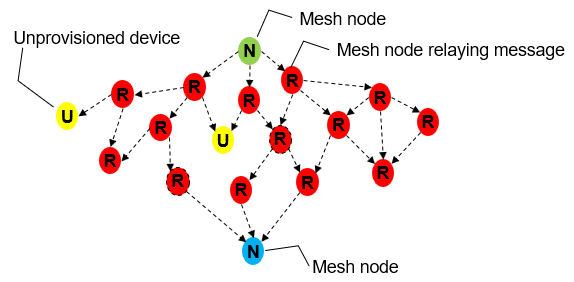
\includegraphics{figures/ble_mesh_structure.png}
\caption{Пример структуры BLE Mesh-сети}
\label{fig:ble_mesh}
\end{figure}

Основные особенности BLE Mesh:
\begin{enumerate}[nosep]
    \item \textbf{Лавинная рассылка сообщений} --- сообщения передаются по сети путём ретрансляции (flooding), при которой узлы пересылают полученные пакеты дальше, расширяя область покрытия.

    \item \textbf{Роли устройств} --- устройства в сети делятся на:
    \begin{itemize}[nosep]
        \item ненастроенные устройства (unprovisioned devices);
        \item узлы (nodes), являющиеся полноправными участниками сети;
        \item ретрансляторы (relay nodes), обеспечивающие пересылку сообщений.
    \end{itemize}

    \item \textbf{Процесс ввода в сеть} --- добавление устройства в сеть осуществляется процедурой provisioning, в ходе которой устройству назначаются сетевые параметры и ключи безопасности.

    \item \textbf{Безопасность} --- для защиты сообщений используются сетевые ключи (network keys), обеспечивающие аутентификацию и шифрование трафика.

    \item \textbf{Модельная архитектура} --- функциональность узлов определяется набором моделей (models), описывающих поведение устройства (например, управление освещением, датчики, таймеры и сцены).
\end{enumerate}

Mesh-сети Bluetooth стандартизированы организацией Bluetooth SIG ~\cite{bluetooth_mesh_spec} и ориентированы на применение в системах автоматизации и управления, таких как:
\begin{itemize}[nosep]
    \item системы «умного дома»;
    \item промышленная автоматизация;
    \item сети датчиков;
    \item управление освещением;
    \item мониторинг и отслеживание объектов.
\end{itemize}

В отличие от скаттернета, BLE Mesh не требует строгой синхронизации между узлами и обеспечивает более высокую масштабируемость и отказоустойчивость за счёт децентрализованной передачи данных.

Таким образом, технология Bluetooth поддерживает гибкий набор топологий, позволяющий строить сети различной сложности --- от простейших соединений точка--точка до масштабируемых Mesh сетей.


\subsection{Анализ областей применения Bluetooth в современных беспроводных сетях}

Технология Bluetooth за время своего развития превратилась в универсальный стандарт для организации короткодистанционных беспроводных сетей. Благодаря открытой спецификации и широкой поддержке со стороны производителей, Bluetooth применяется в различных областях — от пользовательской электроники до промышленных систем и Интернета вещей.

\subsubsection{Персональные сети и периферийные устройства}

Одним из основных направлений применения Bluetooth является организация персональных беспроводных сетей (WPAN). Технология используется для подключения периферийных устройств, таких как клавиатуры, мыши, принтеры и контроллеры, к компьютерам и мобильным устройствам. Использование профилей HID, BPP и SPP позволяет отказаться от проводных соединений, повышая удобство эксплуатации и мобильность пользователей.

\subsubsection{Аудио и мультимедийные системы}

Bluetooth широко применяется для передачи аудиосигналов. Профили A2DP и AVRCP обеспечивают потоковую передачу стереозвука и управление воспроизведением, а профили HSP и HFP используются для голосовой связи. Современные версии стандарта (начиная с Bluetooth 5.2) поддерживают технологию LE Audio, которая обеспечивает более высокое качество звука при меньшем энергопотреблении и позволяет реализовать многопоточное аудио и широковещательную передачу звука.

\subsubsection{Интернет вещей и носимые устройства}

С появлением Bluetooth Low Energy (BLE) технология стала широко применяться в системах Интернета вещей. Низкое энергопотребление и возможность длительной автономной работы делают BLE оптимальным решением для датчиков, фитнес-трекеров, умных часов и медицинских устройств. Использование протоколов GATT и ATT обеспечивает эффективную передачу небольших объёмов данных в клиент-серверной модели. BLE также применяется в системах умного дома и для позиционирования внутри помещений.

\subsubsection{Промышленность и системы автоматизации}

В промышленности Bluetooth используется для построения сенсорных сетей, мониторинга оборудования и отслеживания объектов. Развитие технологии Bluetooth Mesh позволило создавать масштабируемые сети с большим числом узлов. Такие сети обеспечивают надёжную передачу данных за счёт ретрансляции сообщений между устройствами. Встроенные механизмы шифрования и аутентификации обеспечивают необходимый уровень безопасности при использовании в промышленных системах.

\subsubsection{Транспортные системы}

Bluetooth активно применяется в автомобильной индустрии. Он используется в системах hands-free, потоковой передаче аудио и телематических сервисах. Современные версии стандарта поддерживают улучшенные механизмы определения положения устройств и устойчивость к помехам, что особенно важно в условиях динамической среды.

\subsubsection{Современные тенденции развития}

Современное развитие Bluetooth направлено на повышение энергоэффективности, увеличение дальности и скорости передачи данных, а также расширение функциональности. Новые версии стандарта обеспечивают улучшенное управление соединениями, снижение задержек и поддержку новых сценариев использования. Интеграция с другими технологиями беспроводной связи способствует дальнейшему расширению областей применения Bluetooth.

\subsubsection{Связь с лабораторным стендом}

Разнообразие областей применения Bluetooth обуславливает необходимость его практического изучения. Лабораторный стенд позволяет исследовать различные режимы работы технологии, включая соединения точка--точка, пикосети и BLE-сценарии. В рамках экспериментов возможно анализировать параметры радиоканала, особенности протоколов и влияние помех, что способствует формированию практических навыков работы с беспроводными сетями.

Таким образом, Bluetooth остаётся одной из ключевых технологий для организации короткодистанционных беспроводных соединений и продолжает активно развиваться в соответствии с требованиями современных информационно-коммуникационных систем.

\subsection{Формирование технических требований к учебно-лабораторному стенду}

Переход от теоретического анализа технологии Bluetooth к практической реализации лабораторного комплекса требует формализации технических требований. Они определяют функциональные, аппаратные, программные и эксплуатационные характеристики стенда, обеспечивая его соответствие целям учебного процесса и научно-исследовательской деятельности.

На основе анализа спецификации Bluetooth Core Specification и задач учебного процесса сформирован комплекс требований, структурированный по основным направлениям.

\subsubsection{Функциональные требования}

Стенд должен обеспечивать моделирование и исследование ключевых аспектов работы Bluetooth-сетей:
\begin{enumerate}[nosep]
    \item поддержка топологий «точка--точка» и пикосеть;
    \item возможность работы узлов в ролях ведущего и ведомого;
    \item измерение параметров радиоканала (RSSI, SNR, потери пакетов);
    \item анализ протокольного взаимодействия (L2CAP, RFCOMM, ATT/GATT);
    \item тестирование профилей Bluetooth (SPP, A2DP, HID, GATT);
    \item исследование устойчивости к помехам в диапазоне 2{,}4 ГГц.
\end{enumerate}

\subsubsection{Аппаратные требования}

К аппаратной части стенда предъявляются следующие требования:
\begin{enumerate}[nosep]
    \item Использование микроконтроллеров с поддержкой BR/EDR и BLE (ESP32);
    \item Питание автономных узлов (Li-Po аккумуляторы 3{,}7 В);
    \item Возможность подключения ПК через USB Bluetooth-адаптеры;
    \item Поддержка различных уровней мощности передатчика.
\end{enumerate}

\subsubsection{Программные требования}

Программное обеспечение должно обеспечивать доступ к протоколам Bluetooth и средства анализа:
\begin{enumerate}[nosep]
    \item Использование ОС Linux и стека BlueZ;
    \item Применение инструментов анализа (Wireshark, btmon, hcidump, bluetoothctl);
    \item Использование сред разработки для ESP32 (Arduino IDE, ESP-IDF).
\end{enumerate}

\subsubsection{Эксплуатационные требования}

\begin{enumerate}[nosep]
    \item Доступность и низкая стоимость компонентной базы;
    \item Безопасность эксплуатации;
    \item Масштабируемость системы;
    \item Наличие методического обеспечения лабораторных работ.
\end{enumerate}

\begin{table}[H]
\centering
\caption{Сводная таблица технических требований к учебно-лабораторному стенду}
\label{tab:lab_requirements}
\renewcommand{\arraystretch}{1.3}

\begin{tabularx}{\textwidth}{|X|X|X|}
\hline
\textbf{Категория} & \textbf{Требование} & \textbf{Обоснование} \\
\hline

Функциональные &
Поддержка топологий Bluetooth &
Исследование режимов работы сети \\
\cline{2-3}
&
Измерение параметров радиоканала &
Оценка качества связи \\
\hline

Аппаратные &
Использование ESP32 &
Поддержка BR/EDR и BLE \\
\cline{2-3}
&
Автономное питание &
Мобильность узлов \\
\cline{2-3}
&
USB Bluetooth-адаптеры &
Интеграция ПК в сеть \\
\hline

Программные &
ОС Linux + BlueZ &
Доступ к HCI и инструментам анализа \\
\cline{2-3}
&
Wireshark и утилиты анализа &
Перехват и декодирование пакетов \\
\hline

Эксплуатационные &
Низкая стоимость и масштабируемость &
Использование в учебных лабораториях \\
\hline

\end{tabularx}
\end{table}

Сформированные требования являются основой для проектирования архитектуры стенда, выбора компонентной базы и разработки программного обеспечения, что рассматривается в следующих главах работы.
